\chapter{Training of the CNN}
\label{ch:training_of_the_cnn}
% \todo[inline]{todos, cleanup}

% Building a \acrlong{cnn} requires the design and training of a \acrshort{cnn} model.
Building a \acrlong{cnn} from scratch leaves a lot of design choices and requires multiple steps.
% In a first step, a \acrshort{cnn} architecture is designed and 
% The first step involves the design of the desired \acrshort{cnn} architecture and the tuning of the hyperparameters.
The first step involves the design of the desired \acrshort{cnn} architecture. % todo: remove desired?
In a second step, the labeled dataset is used to fit the \acrshort{cnn} model.
If necessary, the hyperparameters of the \acrshort{cnn} architecture can be tuned in a third step.

% This chapter describes these steps
This chapter describes the dataset generation, the design of the \acrshort{cnn} architecture and the actual training of the \acrshort{cnn} model. % todo: remove actual?

\section{Dataset}
\label{sec:training_of_the_cnn:dataset}

The dataset contains frames of 22 different throwing objects, as shown in table \ref{tab:objects}.
It is fully labeled and consists of more than \num{15000} usable frames with at least \num{485} frames of each object.
All frames were collected over the course of two days during the previous project.
Figure \ref{fig:dataset} shows two example frames from the dataset (the \textit{Stuffed Bunny} and the \textit{Hand Featherball}).

\begin{table}
  \caption{List of the different throwing objects}
  \label{tab:objects}
  \centering
  \begin{tabular}{llll}
    \toprule
    \textbf{Objects} &  &  &  \\
    \midrule
    Nerf Dart & American Football & Table Tennis Ball & Shuttlecock \\ % left to right, top to bottom
    Sporf & Arrow & Hand Featherball & Floorball \\
    Spiky Ball & Tesafilm & Sponge & Red Duplo Brick \\
    Green Duplo Brick & Duplo Figure & Foam Die & Infant Shoe \\
    Stuffed Bunny & Goalkeeper Glove & Hemp Cord & Paper Ball \\
    Beer Cap & Water Bottle &  &  \\
    \bottomrule
  \end{tabular}
\end{table}

\begin{figure}[t]
  \centering
  \begin{subfigure}[b]{0.45\textwidth}
    \centering
    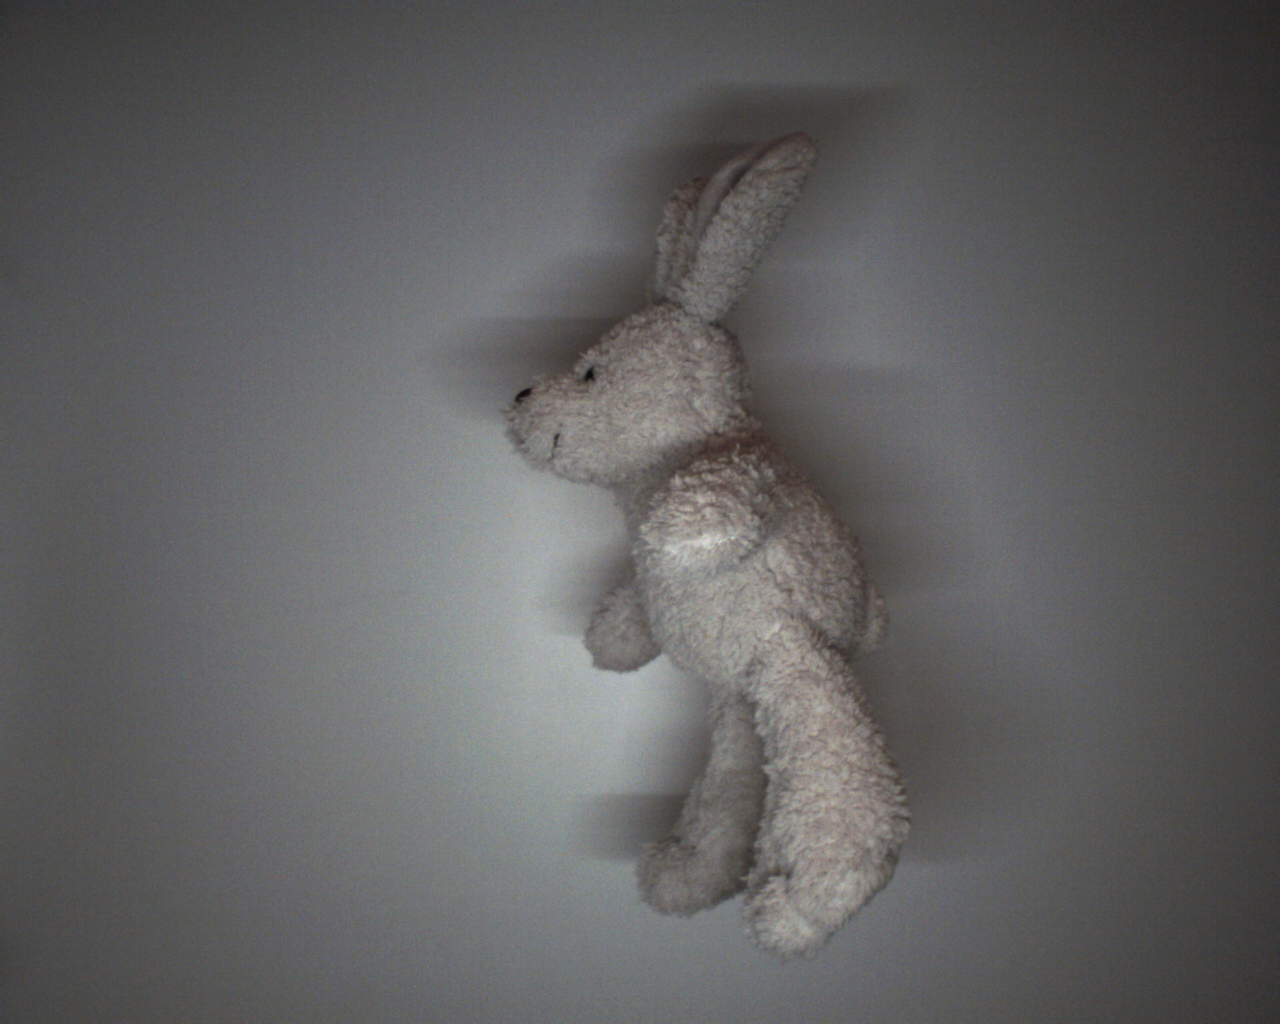
\includegraphics[width=\textwidth]{1574952009_278_10_stuffed-bunny}
    \caption{Stuffed Bunny}
    \label{subfig:dataset_stuffed_bunny}
  \end{subfigure}
  \begin{subfigure}[b]{0.45\textwidth}
    \centering
    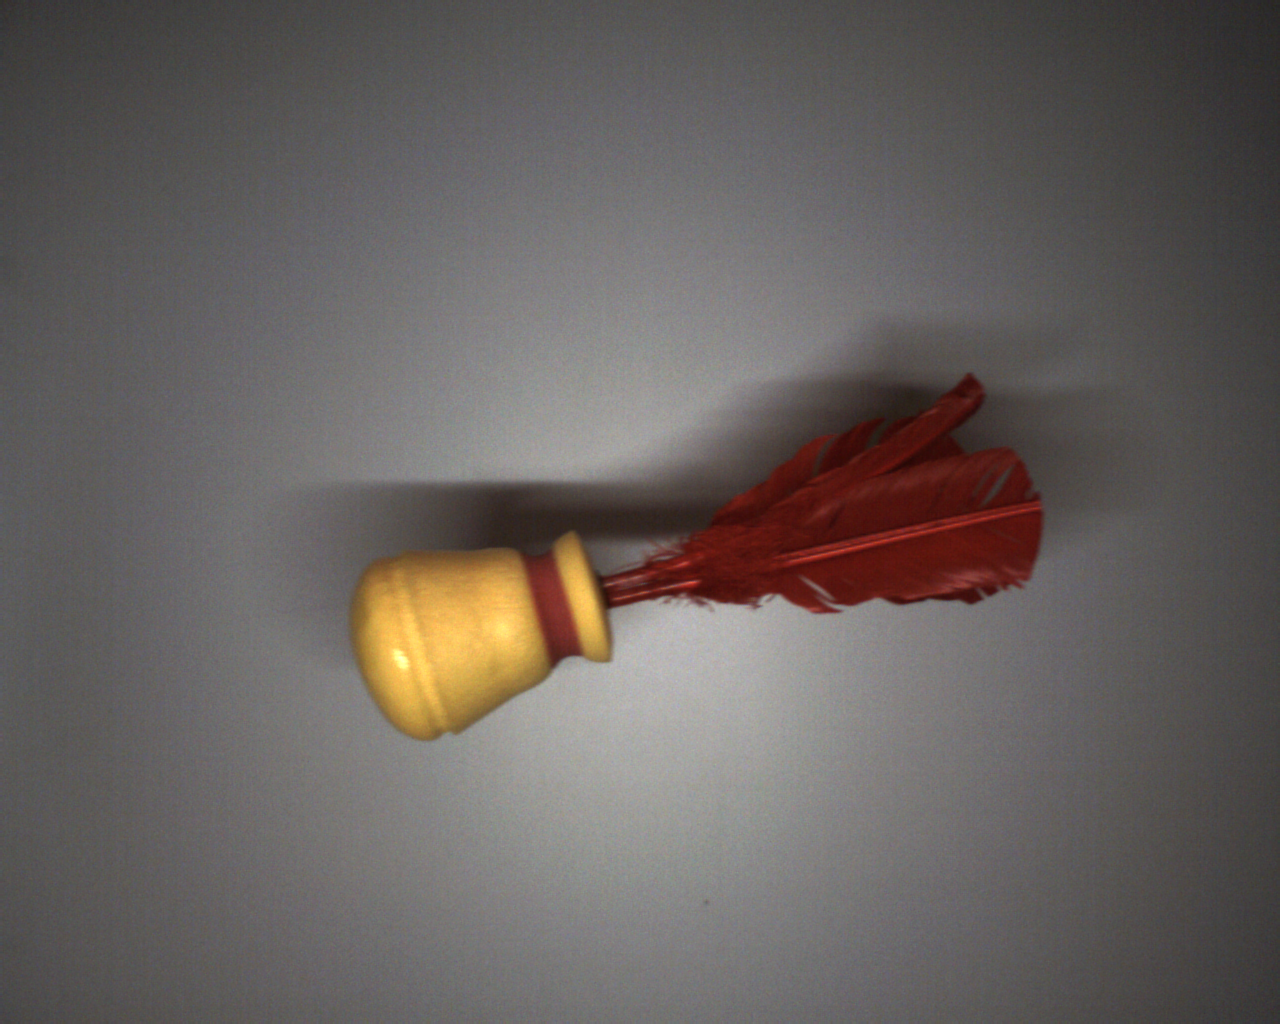
\includegraphics[width=\textwidth]{1574943825_125_8_hand-featherball}
    \caption{Hand Featherball}
    \label{subfig:dataset_hand_featherball}
  \end{subfigure}
  \caption{Two example frames from the dataset}
  \label{fig:dataset}
\end{figure}

% ------------------------------------------------------------------------------------------------------------------------------
\subsection{White Balance}
\label{subsec:training_of_the_cnn:dataset:white_balance}

A notable thing is that on the first day of the data collection, the white balance was performed continuously (every three frames).
This caused the background color of large colored objects to be distorted, as shown in figure \ref{fig:white_balance}.
However, this is not problematic, as noise can improve the generalization and thus reduce overfitting \cite{training_noise}.

\begin{figure}[t]
  \centering
  \begin{subfigure}[b]{0.45\textwidth}
    \centering
    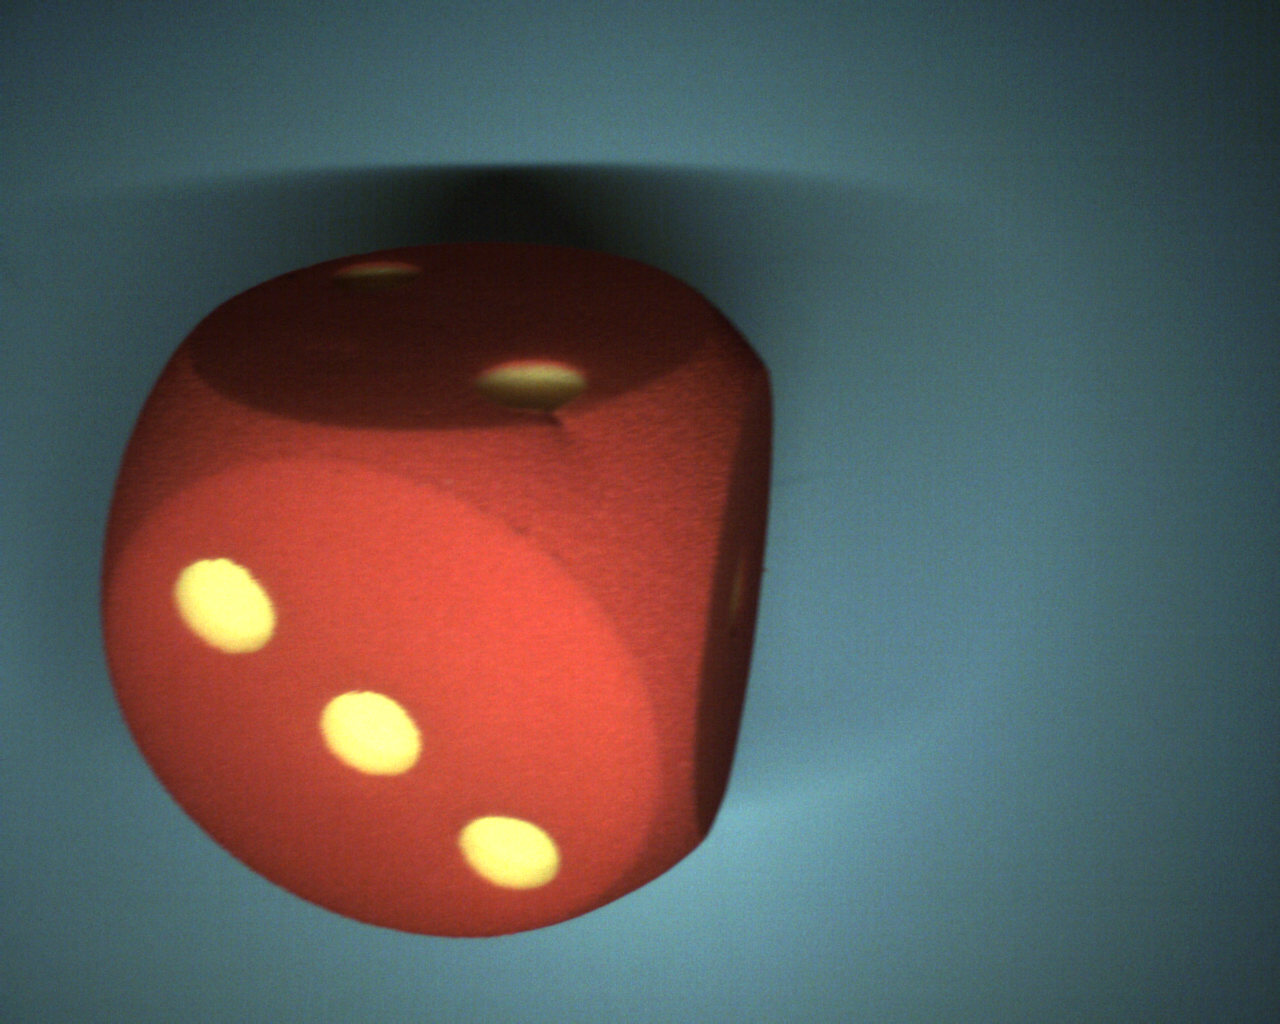
\includegraphics[width=\textwidth]{1574950250_238_9_foam-dice}
    \caption{Continuous white balance}
    \label{subfig:white_balance_first_day}
  \end{subfigure}
  \begin{subfigure}[b]{0.45\textwidth}
    \centering
    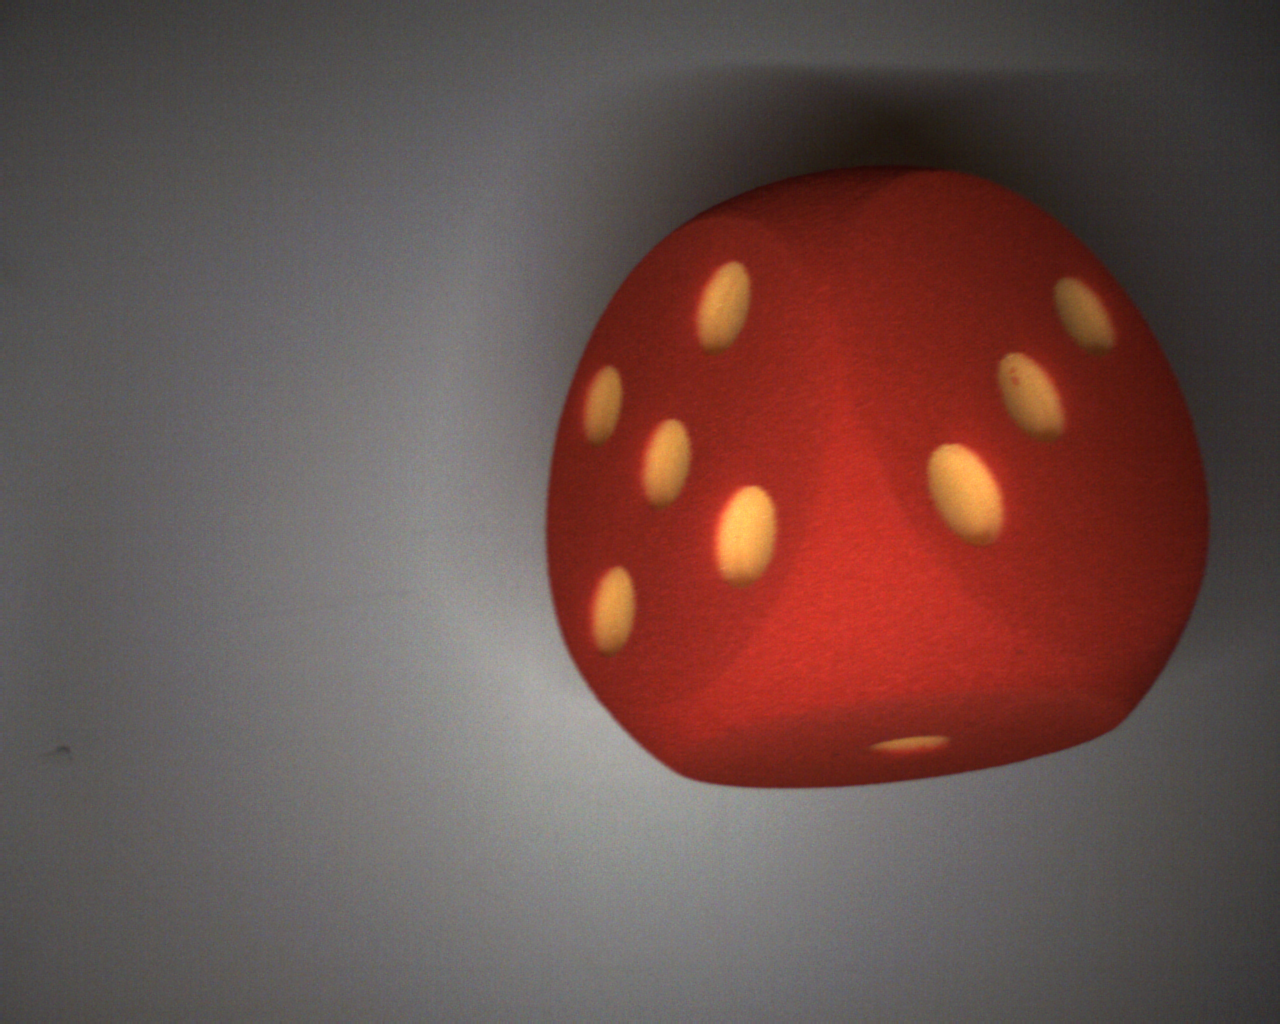
\includegraphics[width=\textwidth]{1575032343_726_8_foam-dice}
    \caption{One-off white balance}
    \label{subfig:white_balance_second_day}
  \end{subfigure}
  \caption{White balance difference between the first (\subref{subfig:white_balance_first_day}) and the second (\subref{subfig:white_balance_second_day}) day}
  \label{fig:white_balance}
\end{figure}

% ------------------------------------------------------------------------------------------------------------------------------
\subsection{Statistics}
\label{subsec:training_of_the_cnn:dataset:statistics}

Figure \ref{fig:statistics} shows the amount of captured frames for each object individually.
It is evident that there are generally more frames of larger objects.
This is, on the one hand, due to the specific implementation of the throw detection mechanism.
On the other hand, the field of view of the camera is not uniformly illuminated (the center is brighter than the edges).
For those reasons, a larger object area is required at the borders to achieve a sufficiently large change in the frame.
However, this also leads to the fact that larger objects are more often only partially in the frame.

The statistics of the dataset reveal that it is slightly imbalanced.
This fact has to be taken into account when creating the various dataset splits (see section \ref{subsec:training_of_the_cnn:dataset:splitting}) that are required for the fitting and evaluation of the model.

An imbalanced dataset can lead to serious problems, e.g. a bias towards the classes with the most samples.
Consider a dataset consisting of only two classes that is imbalanced in such a way that \SI{90}{\percent} of all samples belong to class \texttt{A}.
The fitting process of the classification model will naturally favor class \texttt{A}, since the chance of being right is nine times higher.
The classification could even be independent of the input and always opt for class \texttt{A} (completely ignoring class \texttt{B}).
This obviously terrible classification process would still result in an overall accuracy of \SI{90}{\percent} \cite{training_imbalanced}.

\begin{figure}
  \centering
  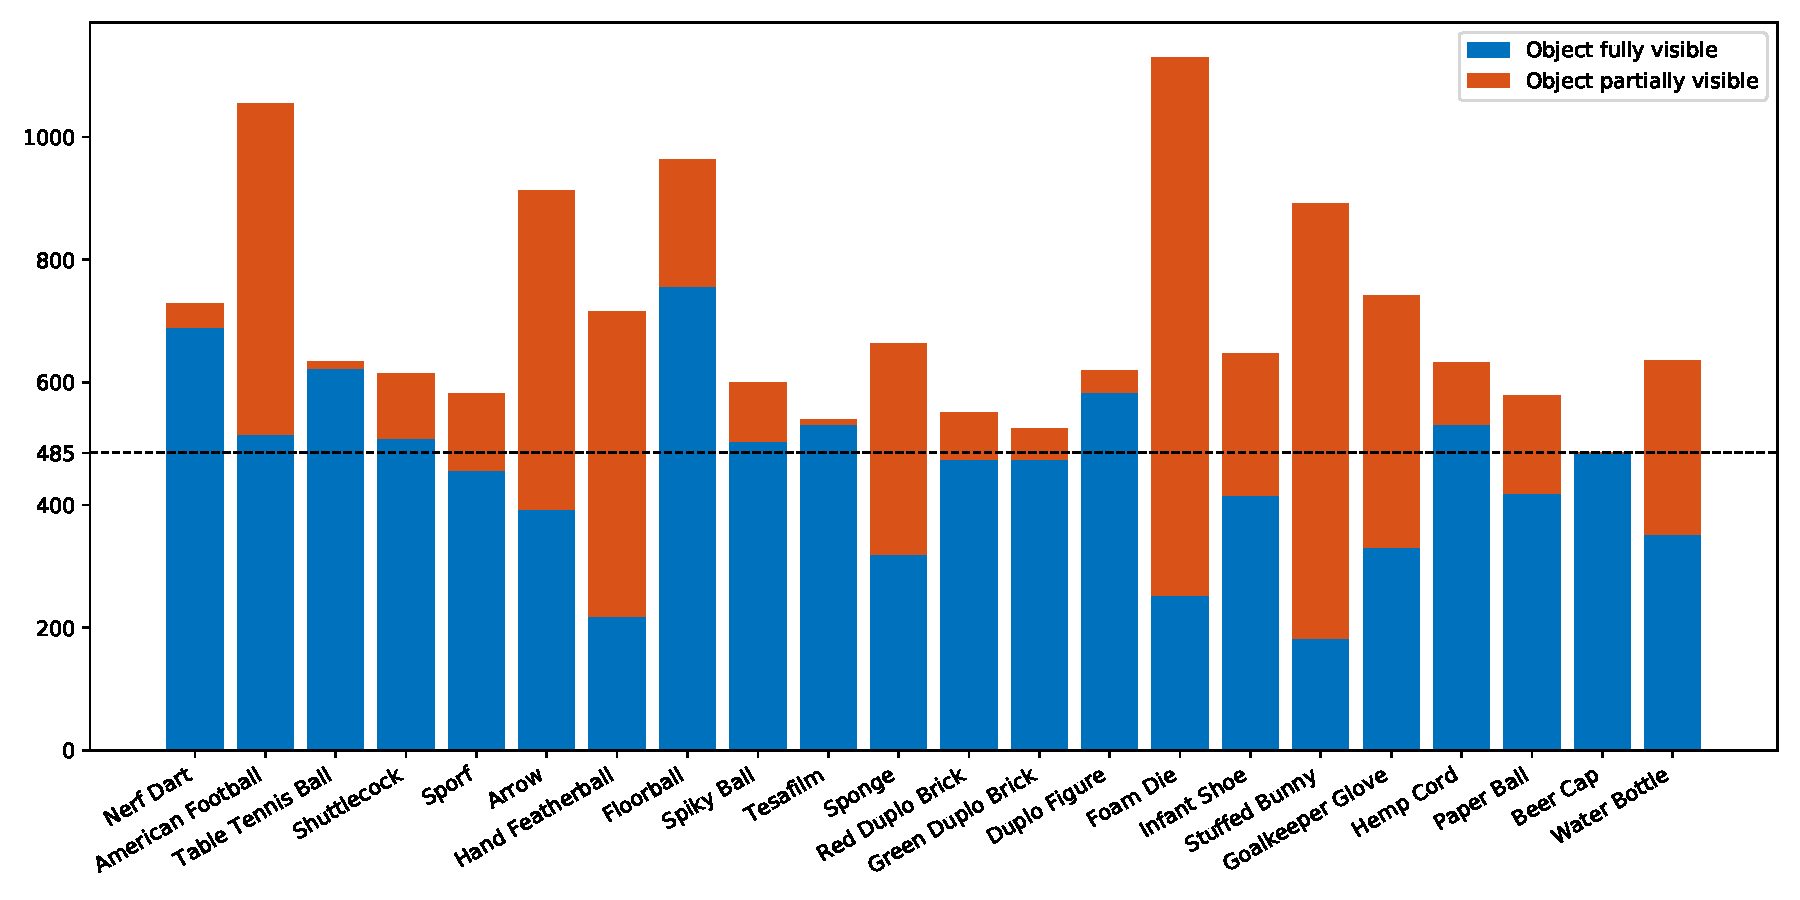
\includegraphics[width=\textwidth]{statistics}
  \caption{Statistics showing the amount of captured frames for each object individually}
  \label{fig:statistics}
\end{figure}

% ------------------------------------------------------------------------------------------------------------------------------
\subsection{Augmentation}
\label{subsec:training_of_the_cnn:dataset:augmentation}

The image dimensions of the individual frames are $1280\times\SI{1024}{px}$ (width $\times$ height) with three color channels (\acrshort{rgb}).
This is an enormous amount of input data for a \acrlong{cnn} and would result in an extremely large amount of mathematical operations to classify even a single frame.
As a result, the classification throughput is reduced and thus the time required to fit the \acrshort{cnn} model is greatly increased.

Another important aspect of the dataset is the fact that it was collected over the course of only two days.
Some objects (e.g. the \textit{Water Bottle}) were even added only on the second day of the data collection.
Real-world observations have shown that the surrounding ambient light and the orientation of an object have a significant influence on the classification performance.
The data collection took place in a relatively dim location and the ambient light did not change much.
The classification performance is therefore much better when there is less ambient light.

Furthermore, the orientation of an object on a frame also impacts the classification performance.
One such problem arises if, for example, the \textit{Shuttlecock} is deliberately thrown with the plastic tail feathers in front of the cork head.
Experiments have shown that this results in a complete misclassification of the object.

For those reasons, a range of image data augmentation techniques are used on the individual frames to improve the real-world classification performance \cite{training_data_augmentation}.
The dataset augmentation is done with the Python script \texttt{dataset\_generator.py}, which uses NumPy as well as the Python implementation of the \acrfull{opencv}.
NumPy provides support for large, multi-dimensional arrays and an assortment of functions to work on these arrays \cite{training_numpy}.
\acrshort{opencv} provides various image transformation functions (e.g. resizing, color space conversions) and conveniently uses NumPy arrays to represent the images \cite{training_opencv_intro}.

% -----------------------
\paragraph{Image Scaling}
To reduce the input data of the \acrshort{cnn} model, the width and height of the individual frames are each scaled down by a factor of four.
This results in an image with the dimensions of $320\times\SI{256}{px}$ (width $\times$ height) and thus in a data reduction of \num{16}.

These dimensions are great because even the important features of the smallest objects are still preserved.
Given that the background of the frames remains more or less the same, a reasonably deep \acrshort{cnn} should have no problems distinguishing between the only \num{22} different classes.

The downsampling is achieved with the use of nearest-neighbor interpolation.
This results in more noise and scaling artifacts than other interpolation methods, such as bilinear or bicubic interpolation.
The scaling artifacts shown in figure \ref{fig:augmentation_downsampling} are the result of aliasing.
The advantages of nearest-neighbor interpolation are its simplicity and fast execution time \cite{training_interpolation}.
Furthermore, the additional noise can improve the generalization and therefore reduce overfitting \cite{training_noise}.

The Python implementation of the image scaling makes use of the \acrshort{opencv} function \texttt{cv2.resize}.
This function is supplied with three arguments: the NumPy array that represents the image, the desired output image size and the interpolation method \cite{training_opencv_resize}.

\begin{figure}
  \centering
  \begin{subfigure}[b]{0.45\textwidth}
    \centering
    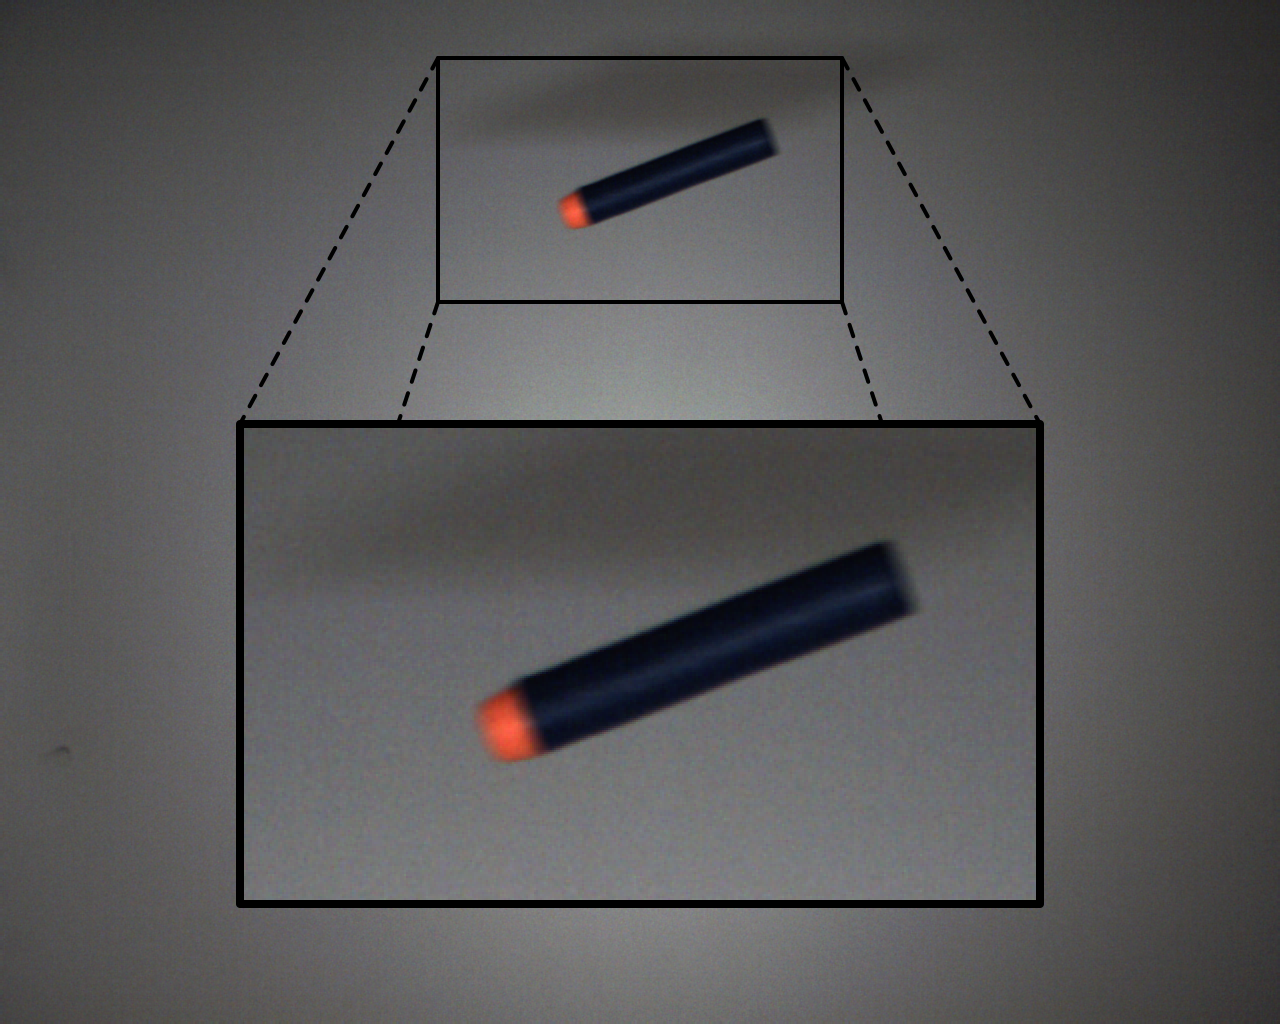
\includegraphics[width=\textwidth]{augmentation_downsampling/1575032863_742_3_nerf-dart_zoom}
    \caption{Original version}
    \label{subfig:ad_original}
  \end{subfigure}
  \begin{subfigure}[b]{0.45\textwidth}
    \centering
    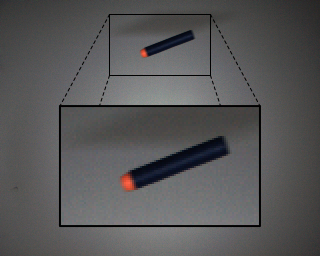
\includegraphics[width=\textwidth]{augmentation_downsampling/1575032863_742_3_nerf-dart_resized_zoom}
    \caption{Scaled-down version}
    \label{subfig:ad_resized}
  \end{subfigure}
  \caption{Example of an original (\subref{subfig:ad_original}) and a scaled-down version (\subref{subfig:ad_resized}) of a frame ($2\times$ inner zoom added to better highlight the difference)}
  \label{fig:augmentation_downsampling}
\end{figure}

% ---------------------
\paragraph{Color Space}
To reduce the dependence on ambient light intensity, the average brightness of the individual frames is changed.
The rounded average brightness $B$ of an image can be calculated using equation \ref{eq:rounded_average_brightness}.
This equation is implemented in Python with the help of the NumPy function \texttt{np.sum}, which computes the sum of all array elements \cite{training_numpy_sum}.

\begin{equation}
  B = \left\lfloor\frac{1}{w\cdot h\cdot c} \cdot \sum\limits_{k=1}^c \sum\limits_{i=1}^h \sum\limits_{j=1}^w \boldsymbol{M}_{ij}^{k} + 0.5\right\rfloor
  \label{eq:rounded_average_brightness}
\end{equation}

where

\begin{tabular}{lll}
  $B$ & = & rounded average brightness \\
  $w$ & = & width of the image \\
  $h$ & = & height of the image \\
  $c$ & = & number of channels \\
  $\boldsymbol{M}^k$ & = & pixel matrix of channel $k$ \\
\end{tabular}
\\

\clearpage

The rounded average brightness of the background was computed at various times of the day and lies between \numrange{85}{160}.
This range includes environments without ambient light as well as environments with indirect sunlight and artificial ambient light.
In the light of these results, a step size of \num{15} was chosen to cover this spectrum of ambient light intensities.
This results in the following six discrete average brightness levels: \num{85}, \num{100}, \num{115}, \num{130}, \num{145} and \num{160}.

Calculating the average brightness of the individual frames is problematic, as the frames contain objects in addition to the background.
For this reason, only the first frame of a throw (which presumably consists mainly of background) is used to compute the average brightness $B_1$.
This value is then used to determine the required brightness offset $\Delta$ for all frames of that throw as shown in equation \ref{eq:offset_calculation}.

\begin{equation}
  \Delta = B_{\text{des}} - B_1
  \label{eq:offset_calculation}
\end{equation}

where

\begin{tabular}{lll}
  $\Delta$ & = & required brightness offset \\
  $B_{\text{des}}$ & = & desired, rounded average brightness \\
  $B_1$ & = & rounded average brightness of the first frame of the throw \\
\end{tabular}
\\

The brightness adjustment is done according to equation \ref{eq:brightness_adjustment}.
The implementation of this equation in Python consists of two steps.
In a first step, the required brightness offset $\Delta$ is added to each pixel of each color channel individually.
The pixel values are 8-bit unsigned integers, which must be in the range between \numrange{0}{255}.
In order to ensure that this range is not exceeded, the values are clipped in a second step.
For this purpose, the NumPy function \texttt{np.clip} is used \cite{training_numpy_clip}.

\begin{equation}
  A_{i,j}^{k} =
  \begin{cases}
    0 & M_{i,j}^{k} + \Delta < 0 \\
    M_{i,j}^{k} + \Delta & 0\leq M_{i,j}^{k} + \Delta\leq 255 \\
    255 & M_{i,j}^{k} + \Delta > 255 \\
  \end{cases}
  \label{eq:brightness_adjustment}
\end{equation}

where

\[
  i = 1, 2, \dots, h \quad \text{and} \quad j = 1, 2, \dots, w \quad \text{and} \quad k = 1, 2, \dots, c
\]

and

\begin{tabular}{lll}
  $A_{i,j}^{k}$ & = & element $i,j$ of the $k$-th channel augmented pixel matrix $\boldsymbol{A}$ \\
  $M_{i,j}^{k}$ & = & element $i,j$ of the $k$-th channel pixel matrix $\boldsymbol{M}$ \\
  $\Delta$ & = & required brightness offset \\
  $h$ & = & height of the image \\
  $w$ & = & width of the image \\
  $c$ & = & number of channels \\
\end{tabular}
\\

Figure \ref{fig:augmentation_brightness} shows an example of the resized frames of the \textit{Water Bottle}, where the brightness levels were adjusted.
For this example, frame \num{12} of throw \num{575} was used.
The rounded average brightness of the first frame of this throw $B_1$ is equal to \num{101}, whereas $B_{12}$ is equal to \num{99}.
Therefore, an additional offset of \num{-2} in regard to the desired brightness levels is expected.
This is due to the fact that the required brightness offset is determined by using the rounded average brightness of the first frame rather than the frame that is being adjusted.

\begin{figure}
  \centering
  \begin{subfigure}[b]{0.15\textwidth}
    \centering
    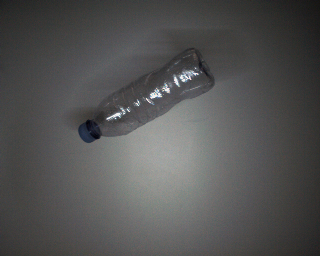
\includegraphics[width=\textwidth]{augmentation_brightness/1575026107_575_12_water-bottle_85}
    \caption{$B = 83$}
    \label{subfig:ab_85}
  \end{subfigure}
  \begin{subfigure}[b]{0.15\textwidth}
    \centering
    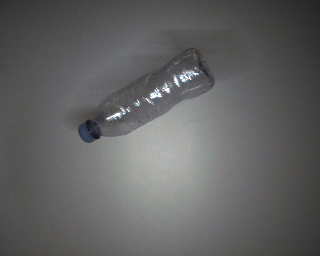
\includegraphics[width=\textwidth]{augmentation_brightness/1575026107_575_12_water-bottle_100}
    \caption{$B = 98$}
    \label{subfig:ab_100}
  \end{subfigure}
  \begin{subfigure}[b]{0.15\textwidth}
    \centering
    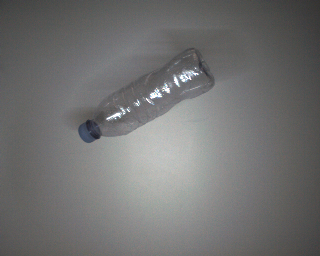
\includegraphics[width=\textwidth]{augmentation_brightness/1575026107_575_12_water-bottle_115}
    \caption{$B = 113$}
    \label{subfig:ab_115}
  \end{subfigure}
  \begin{subfigure}[b]{0.15\textwidth}
    \centering
    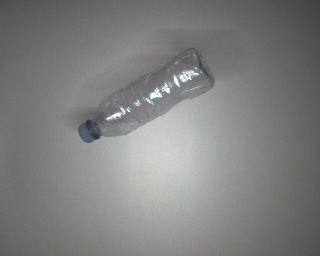
\includegraphics[width=\textwidth]{augmentation_brightness/1575026107_575_12_water-bottle_130}
    \caption{$B = 128$}
    \label{subfig:ab_130}
  \end{subfigure}
  \begin{subfigure}[b]{0.15\textwidth}
    \centering
    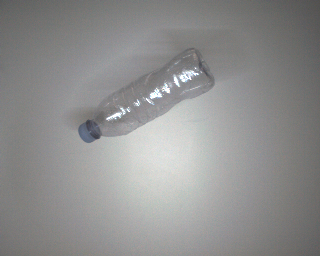
\includegraphics[width=\textwidth]{augmentation_brightness/1575026107_575_12_water-bottle_145}
    \caption{$B = 143$}
    \label{subfig:ab_145}
  \end{subfigure}
  \begin{subfigure}[b]{0.15\textwidth}
    \centering
    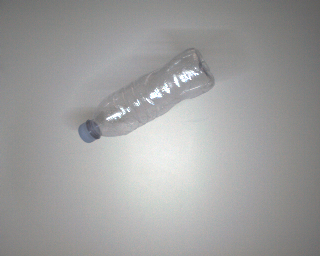
\includegraphics[width=\textwidth]{augmentation_brightness/1575026107_575_12_water-bottle_160}
    \caption{$B = 158$}
    \label{subfig:ab_160}
  \end{subfigure}
  \caption{Examples of resized frames of the \textit{Water Bottle}, where the brightness was adjusted according to the desired brightness levels}
  \label{fig:augmentation_brightness}
\end{figure}

% ------------------
\paragraph{Flipping}
Each frame is flipped vertically and horizontally to improve the orientation-independence of the objects in the frames.
Furthermore, the influence of the shadow that the object casts is decreased.
An example of these reflections is shown in figure \ref{fig:augmentation_flipping}.

The Python implementation uses the \acrshort{opencv} function \texttt{cv2.flip} to flip the frames around the x-axis (vertically) and around the y-axis (horizontally) \cite{training_opencv_flip}.

\begin{figure}
  \centering
  \begin{subfigure}[b]{0.3\textwidth}
    \centering
    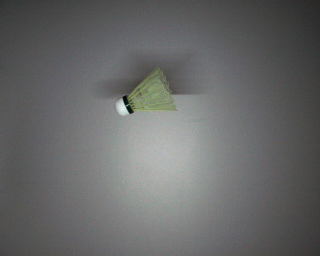
\includegraphics[width=\textwidth]{augmentation_flipping/1575023302_468_9_shuttlecock}
    \caption{Unaugmented}
    \label{subfig:af_resized}
  \end{subfigure}
  \begin{subfigure}[b]{0.3\textwidth}
    \centering
    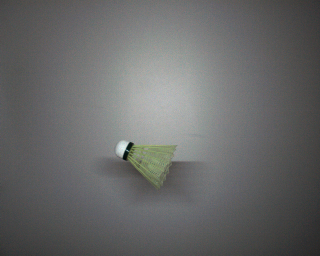
\includegraphics[width=\textwidth]{augmentation_flipping/1575023302_468_9_shuttlecock_v}
    \caption{Vertically flipped}
    \label{subfig:af_vertical}
  \end{subfigure}
  \begin{subfigure}[b]{0.3\textwidth}
    \centering
    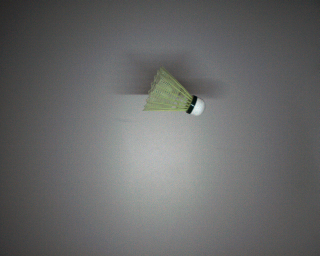
\includegraphics[width=\textwidth]{augmentation_flipping/1575023302_468_9_shuttlecock_h}
    \caption{Horizontally flipped}
    \label{subfig:af_horizontal}
  \end{subfigure}
  \caption{Example of a resized frame of the \textit{Shuttlecock} (\subref{subfig:af_resized}), which was flipped vertically (\subref{subfig:af_vertical}) and horizontally (\subref{subfig:af_horizontal})}
  \label{fig:augmentation_flipping}
\end{figure}

% ------------------------------------------------------------------------------------------------------------------------------
\subsection{Splitting}
\label{subsec:training_of_the_cnn:dataset:splitting}
During the fitting and evaluation process of the \acrshort{cnn} model, three splits of the dataset are required.
These required splits and their respective use is summarized in table \ref{tab:dataset_splits}.

\begin{table}
  \caption{Overview of the required dataset splits \cite{training_datasets}}
  \label{tab:dataset_splits}
  \centering
  \begin{tabular}{llp{10cm}}
    \toprule
    \textbf{Dataset} & \textbf{Split} & \textbf{Description} \\
    \midrule
    \textbf{Training} & \SI{70}{\percent} & The training split is used to fit the model. \\
    \midrule
    \textbf{Validation} & \SI{15}{\percent} & The validation split provides an evaluation of a model fit while tuning hyperparameters of the model. \\
    \midrule
    \textbf{Test} & \SI{15}{\percent} & The test split provides an unbiased evaluation of the final model fit (used to compare fit with other final models). \\
    \bottomrule
  \end{tabular}
\end{table}

It is crucial that the dataset splits are used in the right way.
For example, the validation and the test splits must never be used to fit the model.
Furthermore, it is important to know that the evaluation with the validation split becomes more biased as the classification performance is increased by tuning the hyperparameters of the model.
For this reason, a test split is used to evaluate and compare the final model fit.

The quantization process requires a small unlabeled dataset consisting of \numrange{100}{1000} frames for the calibration of the quantized model.
Seeing that the calibration of the quantized model has many similarities to the tuning of the hyperparameters, the required frames are chosen at random from the validation split.
In total, \num{990} frames are chosen from the validation split (largest possible multiple of the \num{22} classes).
The calibration dataset is thus a subset of the validation dataset without labels.

% ------------------------
\paragraph{Implementation}
The splitting of the dataset is implemented in the Python script \texttt{dataset\_generator.py}, which uses NumPy, \acrshort{opencv} and the standard library.

In a first step, the necessary information about the dataset is fetched from the \acrshort{mysql} database, which is used to store the labels, the file names and other useful metadata.
Table \ref{tab:tab_frames_structure} lists all columns of the database table \texttt{aionfpga.frames}.

\begin{table}
  \caption{Structure of the \acrshort{mysql} database table \texttt{aionfpga.frames}}
  \label{tab:tab_frames_structure}
  \centering
  \begin{tabular}{llll}
    \toprule
    \textbf{Column} & \textbf{Type} & \textbf{Length} & \textbf{Description} \\
    \midrule
    id & \texttt{INT} &  & Sequence number (unique identifier) \\
    timestamp & \texttt{INT} &  & The Unix timestamp at the time of the throw \\
    throwid & \texttt{INT} &  & Throw sequence number \\
    frameid & \texttt{INT} &  & Frame sequence number within a throw \\
    frame & \texttt{VARCHAR} & 255 & The file name of the frame \\
    object & \texttt{VARCHAR} & 255 & The name of the object in the frame (label) \\
    framegood & \texttt{INT} &  & \texttt{0}: frame unusable | \texttt{1}: frame usable \\
    partial & \texttt{INT} &  & \texttt{0}: object fully visible | \texttt{1}: object partially visible \\
    \bottomrule
  \end{tabular}
\end{table}

The slight imbalance in the dataset is mitigated in a next step.
There are several different methods to ensure that the dataset is balanced (e.g. collecting more data, resampling).
For the sake of simplicity, undersampling is used to remove samples from the overrepresented classes \cite{training_imbalanced}.

The actual implementation randomly selects frames from each class.
The number of selected frames is equal to the number of frames in the minority class.
The pseudorandom function used for the selection process is seeded to ensure repeatable results during different tests.
In this case, this results in a loss of about \SI{30.9}{\percent} of the collected frames.

In a third step, the data augmentation discussed in section \ref{subsec:training_of_the_cnn:dataset:augmentation} is performed.
The frames are first resized, then their brightness is adjusted and lastly they are flipped.
The brightness adjustment increases the size of the dataset by a factor of seven and the flipping by a factor of three.
This is due to the fact, that the original frames are preserved as well and results in a total increase of the dataset size by a factor of \num{21}.
Original refers in this case to the resized frames.

The next step is the actual splitting of the dataset.
For this purpose, the entire dataset is shuffled and then split according to table \ref{tab:dataset_splits}.

In a last step, the frames and the labels of the dataset splits are separately saved to the disk.
Due to the sheer number of frames in the dataset splits, the frames are saved in batches of \num{32}.
For this reason, \num{32} frames at a time are stored in a four-dimensional NumPy array of type \texttt{np.uint8} with a shape of $32\times 256\times 320\times 3$ (batch size $\times$ height $\times$ width $\times$ number of color channels).
The \num{22} different labels of the classes (object names) are mapped to a unique number between \num{0} and \num{21}.
This allows for an efficient way to store the labels in one-dimensional NumPy arrays of type \texttt{np.uint8}.
The length of these label arrays is determined by the number of frames in the respective splits.

For each split, both the batch arrays and the label array are saved to the disk in the binary NumPy (\texttt{.npy}) file format \cite{training_numpy_format}.
This allows for fast loading of the dataset from the disk \cite{training_numpy_npy}.

Listing \ref{lst:save_batches} shows the function \texttt{save\_batches}, which implements this last step.

\begin{lstlisting}[style=python, caption={Python function \texttt{save\_batches} to save the batch arrays and the label array}, label=lst:save_batches]
def save_batches(frames_name, labels_name, dst, frame_names, batch_size):

  num_frames = len(frame_names)
  num_batches = math.ceil(num_frames / batch_size)

  labels = np.empty((num_frames,), dtype=np.uint8)
  for idx in range(num_batches):
    start = idx * batch_size
    end = start + batch_size
    frame_names_slice = frame_names[start:end]

    frames = np.empty((len(frame_names_slice),) + fh.inf_shape, dtype=np.uint8)
    for i, frame in enumerate(frame_names_slice):
      obj_san = frame.split('_')[3]
      label = fh.objects_san.index(obj_san)
      frames[i] = cv2.imread(str(fh.dir_frames_augmented / f'{frame}.png'))
      labels[idx * batch_size + i] = label

    np.save(dst / f'{frames_name}_batch_{idx}_of_{num_batches}.npy', frames)

  np.save(dst / f'{labels_name}.npy', labels)
\end{lstlisting}

% ----------------
\paragraph{Result}
The toal number of frames after the augmentation is equal to \num{224070}.
The final training dataset consists of \num{156882} frames and requires \SI{35.91}{GiB} of disk space.
The validation and test datasets each comprise of \num{33594} frames and require \SI{15.38}{GiB} of disk space together.

\section{Architecture}
\label{sec:training_of_the_cnn:architecture}
% \todo[inline]{too much 'the', citations, todos, cleanup}

% Designing a \acrlong{cnn} architecture from scratch  (e.g. types and number of layers, number of filters, kernel size).
% The design of a \acrlong{cnn} architecture from scratch involves choosing the types of layers and their arrangement as well as many hyperparameters.
% Designing a \acrlong{cnn} architecture from scratch involves choosing the types of layers and their arrangement as well as many hyperparameters.
Designing a \acrlong{cnn} architecture from scratch requires choosing the types of layers and their arrangement as well as many hyperparameters.
% There are infinitely many ways to design a \acrlong{cnn} architecture from scratch (e.g. types of layers and their arrangement, many hyperparameters).
% There is currently no perfect way to design a good model and a lot of trial and error is 
For this reason, a lot of trial an error is involved in the design process of an adequate model \cite{training_arch_design}.
% For this reason, there are a infinitely many ways to design an adequate model and a lot of trial an error is involved in the design process of an adequate model. % todo: cite http://www.isikdogan.com/blog/how-to-design-a-convolutional-neural-network.html
There are, however, certain design principles that work really well \cite{training_arch_hyper}:
% the deeper in the net, the more filters and lower spatial dimensions (max pooling)

\begin{enumerate}
  % \item Starting with a low number of filters and increasing 
  \item Starting with a low number of filters (high-level feature detection)
  \item Increasing the number of filters towards the end (low-level feature detection)
  \item Decreasing the spatial dimensions of the feature maps towards the end
  \item Using kernel sizes of $3\times 3$, $5\times 5$ or $7\times 7$ for convolutional layers
  % \item Using kernel sizes of $2\times 2$ or $3\times 3$ with a stride of two for max-pooling layers
  \item Using pool sizes of $2\times 2$ or $3\times 3$ with a stride of two for max-pooling layers
  \item Adding additional layers until the model is overfitting
  \item Using state-of-the-art networks as inspiration
\end{enumerate}

% A summary of all the layers is listed in table \ref{tab:arch}.
A summary of all the layers of the final \acrshort{cnn} architecture is listed in table \ref{tab:arch}.
% A kernel size of $5\times 5$ is chosen for the first convolutional layer
% Due to the large input shape of the frames, a larger kernel size of $5\times 5$ is chosen for the first convolutional layer.
% The first convolutional layer uses \num{16} filters and a larger kernel size of $5\times 5$ due to the large input shape of the frames.
The first convolutional layer uses only \num{16} filters and a larger kernel size of $5\times 5$ due to the large dimensions of the input images.
All other convolutional layers use a kernel size of $3\times 3$ while steadily increasing the number of used filters up to \num{128}.
% only max pooling is used
% max amount of poooling layers used (iage size of 5x4)
% The architecture uses the maximum amount of max-pooling layers for the given input shape.
% The designed architecture uses six max-pooling layers with a kernel size of $2\times 2$ and a stride of two.
The designed architecture uses six max-pooling layers with a pool size of $2\times 2$ and a stride of two.
% This reduces the spatial dimensions of the input feature maps down to $4\times 5$.
This reduces the spatial dimensions of the feature maps to $4\times 5$ (height $\times$ width).
% The fully-connected layer \texttt{fc8} is several times larger than the output layer \texttt{fc9}.
The output of the fully-connected layer \texttt{fc8} is about the size of the output layer \texttt{fc9} squared.
This allows the output layer to combine many of the different high-level features to create a confident prediction.
% This allows the output layer a variety of combinations of the different high-level features 

% no more layers were added (was simply not necessary, it converged incredible fast)
Even though the model was not yet overfitting, no additional layers were added.
% The reason for this is that the classification performance is already exceptional with the current architecture.
% The reason for this is that with the current architecture the classification performance is already exceptional (see section \ref{sec:training_of_the_cnn:training}).
The reason for this is that with the current architecture the classification performance is already exceptional.

% number of parameter relatively low compared to state-of-the-art networks
% compare this and back up with the citation below
% Furthermore, the number of trainable parameters (weights) is relative low compared to state-of-the-art networks (e.g. VGG, ResNet, Inception) \cite{}. % todo: cite https://keras.io/api/applications/
Furthermore, the number of trainable parameters (weights) is relative low compared to state-of-the-art networks like VGG, ResNet or Inception \cite{training_arch_keras}.
This increases the throughput considerably, as less mathematical operations are required.
% talk about the importance of keeping the parameters of the first fc layer down!
% The keys to keeping the total number of trainable parameter low are the shape of the feature maps of the last convolutional layer and the artifical output neurons of the first dense layer.
% This is evident when analyzing the number of trainable parameters listed in table \ref{tab:arch}.
The key to keeping the total number of trainable parameter low is evident when analyzing table \ref{tab:arch}.
% A whopping \num{1311232} of the \num{1614486} total weights stem from the connection between those layers.
% A whopping \num{1311232} of the \num{1614486} total weights can be attributed to the connection between these layers.
A whopping \num{1311232} of the \num{1614486} total weights can be attributed to the connection between the feature maps of the last convolutional layer \texttt{conv7} and the artificial output neurons of the first dense layer \texttt{fc8}.
This accounts for \SI{81.22}{\percent} of all trainable parameters.
% This is the reason why the spatial dimensions of the feature maps should be decreased towards the end.
For this reason the spatial dimensions of the feature maps should be decreased towards the end.
% For this reason the spatial dimensions of the feature maps should decrease towards the end. % todo: maybe use this?

\begin{table}
  \caption{Layers of the \acrshort{cnn} architecture}
  \label{tab:arch}
  \centering
  \begin{tabular}{lllllll}
    \toprule
    \textbf{Layer} & \textbf{Type} & \textbf{Activation} & \textbf{Filters} & \textbf{Kernel} & \textbf{Output Shape} & \textbf{Param \#} \\
    \midrule
    \textbf{conv1} & \texttt{Conv2D} & \acrshort{relu} & \num{16} & $5\times 5$ & $256\times 320\times 16$ & \num{1216} \\
    \textbf{pool1} & \texttt{MaxPooling2D} &  &  & $2\times 2$ & $128\times 160\times 16$ & \num{0} \\
    \midrule
    \textbf{conv2} & \texttt{Conv2D} & \acrshort{relu} & \num{32} & $3\times 3$ & $128\times 160\times 32$ & \num{4640} \\
    \textbf{pool2} & \texttt{MaxPooling2D} &  &  & $2\times 2$ & $64\times 80\times 32$ & \num{0} \\
    \midrule
    \textbf{conv3} & \texttt{Conv2D} & \acrshort{relu} & \num{32} & $3\times 3$ & $64\times 80\times 32$ & \num{9248} \\
    \textbf{pool3} & \texttt{MaxPooling2D} &  &  & $2\times 2$ & $32\times 40\times 32$ & \num{0} \\
    \midrule
    \textbf{conv4} & \texttt{Conv2D} & \acrshort{relu} & \num{64} & $3\times 3$ & $32\times 40\times 64$ & \num{18496} \\
    \textbf{pool4} & \texttt{MaxPooling2D} &  &  & $2\times 2$ & $16\times 20\times 64$ & \num{0} \\
    \midrule
    \textbf{conv5} & \texttt{Conv2D} & \acrshort{relu} & \num{64} & $3\times 3$ & $16\times 20\times 64$ & \num{36928} \\
    \textbf{pool5} & \texttt{MaxPooling2D} &  &  & $2\times 2$ & $8\times 10\times 64$ & \num{0} \\
    \midrule
    \textbf{conv6} & \texttt{Conv2D} & \acrshort{relu} & \num{128} & $3\times 3$ & $8\times 10\times 128$ & \num{73856} \\
    \textbf{pool6} & \texttt{MaxPooling2D} &  &  & $2\times 2$ & $4\times 5\times 128$ & \num{0} \\
    \midrule
    \textbf{conv7} & \texttt{Conv2D} & \acrshort{relu} & \num{128} & $3\times 3$ & $4\times 5\times 128$ & \num{147584} \\
    \midrule
    \textbf{flatten} & \texttt{Flatten} &  &  &  & \num{2560} & \num{0} \\
    \textbf{fc8} & \texttt{Dense} & \acrshort{relu} &  &  & \num{512} & \num{1311232} \\
    \textbf{fc9} & \texttt{Dense} &  &  &  & \num{22} & \num{11286} \\
    \bottomrule
  \end{tabular}
\end{table}

\subsection{Visualization}
\label{subsec:training_of_the_cnn:architecture:visualization}
% The final architecture of the \acrshort{cnn} model is visualized in figure \ref{fig:arch}.
% Figure \ref{fig:arch} shows the final architecture of the \acrshort{cnn} model.
% Figure \ref{fig:arch} visualizes the final architecture of the \acrshort{cnn} model listed in table \ref{tab:arch}.
Figure \ref{fig:arch} visualizes the final architecture of the \acrshort{cnn} model.
The visualization was created with Ti\textit{k}Z and the help of the open-source repository \textit{PlotNeuralNetwork} \cite{training_arch_plot}.
% The final architecture of the \acrshort{cnn} model shown in figure \ref{fig:arch} was visualized with the help of the open source tool PlotNeuralNetwork \cite{}.
% todo: cite https://github.com/HarisIqbal88/PlotNeuralNet or https://doi.org/10.5281/zenodo.2526396
% Haris Iqbal. (2018, December 25). HarisIqbal88/PlotNeuralNet v1.0.0 (Version v1.0.0). Zenodo. http://doi.org/10.5281/zenodo.2526396

% todo: lots of sentences starting with 'the'
The boxes represent the outputs of the different layers.
% The light orange boxes with darker orange bands represent convolutional layers with the \acrshort{relu} activation function.
% The light orange boxes with darker orange bands represent convolutional layers, which use the \acrshort{relu} activation function.
% The light orange boxes with darker orange bands represent the feature maps of the convolutional layers, which use the \acrshort{relu} activation function.
% The light orange boxes with darker orange bands represent the feature maps of the convolutional layers with the \acrshort{relu} activation function applied.
% The light orange boxes represent the feature maps of the convolutional layers and the darker orange bands indicate that the \acrshort{relu} activation function is applied.
On the one hand, the light orange boxes represent the feature maps of the convolutional layers and, on the other hand the purple boxes represent the artificial output neurons of the dense layers.
The darker colored bands on the boxes indicate that the \acrshort{relu} activation function is applied.
% darker orange bands indicate that the \acrshort{relu} activation function is applied.
% Again, the darker purple band of \texttt{fc8} indicates that the \acrshort{relu} activation function is applied
The red boxes represent max-pooling layers, which decrease the spatial dimensions.
% The dashed lines between the output of \texttt{conv7} and \texttt{fc8} depict the flattening and the dense connection between of the convolutional layer
% The dashed lines between the output of \texttt{conv7} and \texttt{fc8} depict the flattening as well as the dense connection between the layer outputs.
% The dashed lines between the output of \texttt{conv7} and \texttt{fc8} depict the flattening as well as the dense connection.
The dashed lines between the output of \texttt{conv7} and \texttt{fc8} depict the flattening in addition to the dense connection.

\begin{figure}
  \centering
  \includegraphics[width=\textwidth]{arch}
  \caption{Final architecture of the \acrlong{cnn}}
  \label{fig:arch}
\end{figure}

\subsection{Implementation}
\label{subsec:training_of_the_cnn:architecture:implementation}
% The dataset augmentation is done with the Python script \texttt{dataset\_generator.py}, which uses NumPy as well as the Python implementation of the \acrfull{opencv}.
% The \acrshort{cnn} architecture is implemented in the Python script \texttt{cnn.py}, as shown in listing \ref{lst:arch}.
The \acrshort{cnn} architecture is defined in the Python script \texttt{cnn.py}, as shown in listing \ref{lst:arch}.
% implementation with TF 2.2.0, Keras backend/frontend?!, PYthon
% Implementation of the Keras API meant to be a high-level API for TensorFlow.
% The script uses the open-source software library TensorFlow v2.2.0, which serves as the default backend for Keras
% The script uses the open-source software library TensorFlow v2.2.0, along with the high-level Keras \acrshort{api} in the \texttt{tf.keras} module \cite{}. % todo: cite https://www.tensorflow.org/versions/r2.2/api_docs/python/tf/keras
The script uses the open-source software library TensorFlow v2.2.0, along with the high-level Keras \acrshort{api} implemented in the \texttt{tf.keras} module \cite{training_arch_tf_keras}.
% todo: or maybe cite https://www.tensorflow.org/api_docs/python/tf/keras
% easy implementation with the sequential model
To define the architecture a \texttt{Sequential} model is used to arrange the desired layers in a plain stack \cite{training_arch_tf_keras_seq}.

\begin{lstlisting}[style=python, caption={Sequential model}, label=lst:arch]
# Convolutional Neural Network Architecture
# Convolution layers
model = models.Sequential()
model.add(layers.Conv2D(16, (5, 5), padding='same', activation='relu', input_shape=fh.inf_shape))
model.add(layers.MaxPooling2D((2, 2)))
model.add(layers.Conv2D(32, (3, 3), padding='same', activation='relu'))
model.add(layers.MaxPooling2D((2, 2)))
model.add(layers.Conv2D(32, (3, 3), padding='same', activation='relu'))
model.add(layers.MaxPooling2D((2, 2)))
model.add(layers.Conv2D(64, (3, 3), padding='same', activation='relu'))
model.add(layers.MaxPooling2D((2, 2)))
model.add(layers.Conv2D(64, (3, 3), padding='same', activation='relu'))
model.add(layers.MaxPooling2D((2, 2)))
model.add(layers.Conv2D(128, (3, 3), padding='same', activation='relu'))
model.add(layers.MaxPooling2D((2, 2)))
model.add(layers.Conv2D(128, (3, 3), padding='same', activation='relu'))

# Dense layers
model.add(layers.Flatten())
model.add(layers.Dense(512, activation='relu'))
model.add(layers.Dense(22))
\end{lstlisting}

\section{Training}
\label{sec:training}



